\section{LHCb Upgrade}
\subsection{Introduction}

The LHCb experiment is designed to detect the decay of long-lived particles: beauty and charmed mesons. As so, it is naturally suited for the search of BSM long-lived particles in a range of mass and lifetime not too dissimilar. It is the only LHC experiment to be fully instrumented in the forward region $2<\eta<5$, where $B$ and $D$ decays are abundant and their decay length is enhanced thanks to the boost. In this region, detector occupancy is extremely high and therefore during LHC Run 1 and Run 2, the experiment has been run at reduced luminosity compared to ATLAS and CMS. However, an upgrade of the detector is foreseen to run at a five times larger luminosity ($2\times 10^{33}\text{cm}^{-2}\text{s}^{-1}$) in LHC Run 3 (starting in 2021) while maintaining or improving the current physics performance. This first upgrade phase (Phase-I) will entail a novel trigger paradigm where all sub-detectors are fast enough to be read out in real time and the first trigger level is done in software. This trigger scheme is  extremely flexible and offers a great opportunity for searches of striking signatures like those of BSM long-lived particles. This upgrade comes earlier than the ATLAS and CMS upgrades planned for the HL-LHC phase (starting in 2026) and will be followed by a Phase-II upgrade (planned for 2031) to run at an even more challenging luminosity of $\sim 2\times 10^{34}\text{cm}^{-2}\text{s}^{-1}$. 
%CVS: mention LHCb Consolidation phase?

Section~\ref{sec:ulhcbperf} gives a brief overview of the (Phase I) upgraded-LHCb detector-design and the expected performance of sub-detectors. 
An overview of its capabilities in the context of LLP searches is given in Section~\ref{sec:ulhcbphys} with a few example signatures. 
Finally, an overlook of the plans for the Phase-II upgrade and some thoughts on the opportunities given by putative additional detector features are reported in Section~\ref{sec:ulhcbphaseii}.



\subsection{LHCb detector and trigger upgrade for Run 3 (Phase I)}
\label{sec:ulhcbperf}

In LHC Run 3, LHCb plans to take data at an instantaneous luminosity of $2\times 10^{33}\text{cm}^{-2}\text{s}^{-1}$, a factor five higher compared to the current one. The LHCb detector needs to be upgraded to cope with the higher radiation dose and most importantly to avoid the saturation of the trigger rate and exploit the higher luminosity. The main bottleneck in the current trigger is in the first stage, which reduces the accepted rate from 30 to 1 MHz directly at hardware level. For the upgrade, the hardware trigger will be removed and the full event will be read out at the bunch crossing rate of the LHC (40~MHz), with a very flexible software-based trigger. \\

\begin{table}[h!]
    \centering
    \begin{tabular}{lrrr}
         & Current Conditions & Phase-I Conditions & Phase-II Conditions \\
        \hline
        $\cal L$ & $4 \times 10^{32} \text{cm}^{-2}\text{s}^{-1}$ & $2 \times 10^{33} \text{cm}^{-2}\text{s}^{-1}$ & $2 \times 10^{34} \text{cm}^{-2}\text{s}^{-1}$\\
        $\int_{ } \cal L$   & $8 \text{fb}^{-1}$ by 2019 & $50 \text{fb}^{-1}$ by 2030 & $300 \text{fb}^{-1}$ by 203x \\
        $\sqrt{\text{s}}$       & 13 TeV & 14 TeV & 14 TeV \\
        $\mu$    & 1.1 & 5.5 & 50 \\
        \hline
    \end{tabular}
    \caption{LHCb current and upgraded operating conditions. Instantaneous luminosity $\cal L$, integrated luminosity $\int_{ } \cal L$, $pp$ collision energy $\sqrt{s}$ and average number of visible interactions $\mu$ are listed.}
    \label{tab:cond}
\end{table}

Table \ref{tab:cond} summarises the current and upgraded conditions of the detector. To cope with the larger occupancy and higher rate of the upgraded detector, the electronics of all the sub-detectors have to be upgraded and some sub-detectors fully replaced. This is the case for the whole tracking system which plays a crucial role in LLP searches.\\

The upgraded tracking system consists of the VErtex LOcator (VELO), surrounding the interaction point, the Upstream Tracker (UT), a tracking station placed before the magnet, and the Scintillating Fibers tracker (SciFi), three stations after the magnet. 
In the VELO~\cite{LHCb-TDR-013}, the current strips will be replaced by pixel detectors, with a custom developed ASIC (VeloPix) able to withstand a maximum hit rate of 900 Mhits/s/ASIC. The UT~\cite{LHCb-TDR-015} is composed of four silicon micro-strip planes, with finer granularity and larger acceptance compared to the current tracker. Each station of the SciFi has four planes of 2.5 m long scintillating fibres read out by silicon photo-multipliers.

The upgrade components most important for LLP searches are probably the  VELO, the tracking and the software trigger. In the following subsections a brief description of their design and capabilities is given.


\subsubsection{Upgrade VELO}
The VELO plays a fundamental role in LLP searches at LHCb: together with the large boost particles usually get in the forward direction, a very precise measurement of the LLP vertex position allows LHCb to access very low lifetimes that are often not accessible at ATLAS and CMS.

In upgrade conditions, the number of tracks and primary vertices will increase by about a factor five, making it much more difficult to identify displaced vertices close to the beam-line, left alone to do it in real time.
The VELO was thus completely redesigned to cope with the new conditions, maintain high physics performance and allow real time readout for the software trigger. The new VELO has a pixel rather than strip geometry and its distance from the LHC beams is reduced from 8 to 5 mm. This allows to improve the vertex resolution (\ref{fig:ulhcb_pvres}) and to reduce the rate of unphysical (ghost) tracks.

\begin{figure}[h]
\centerline{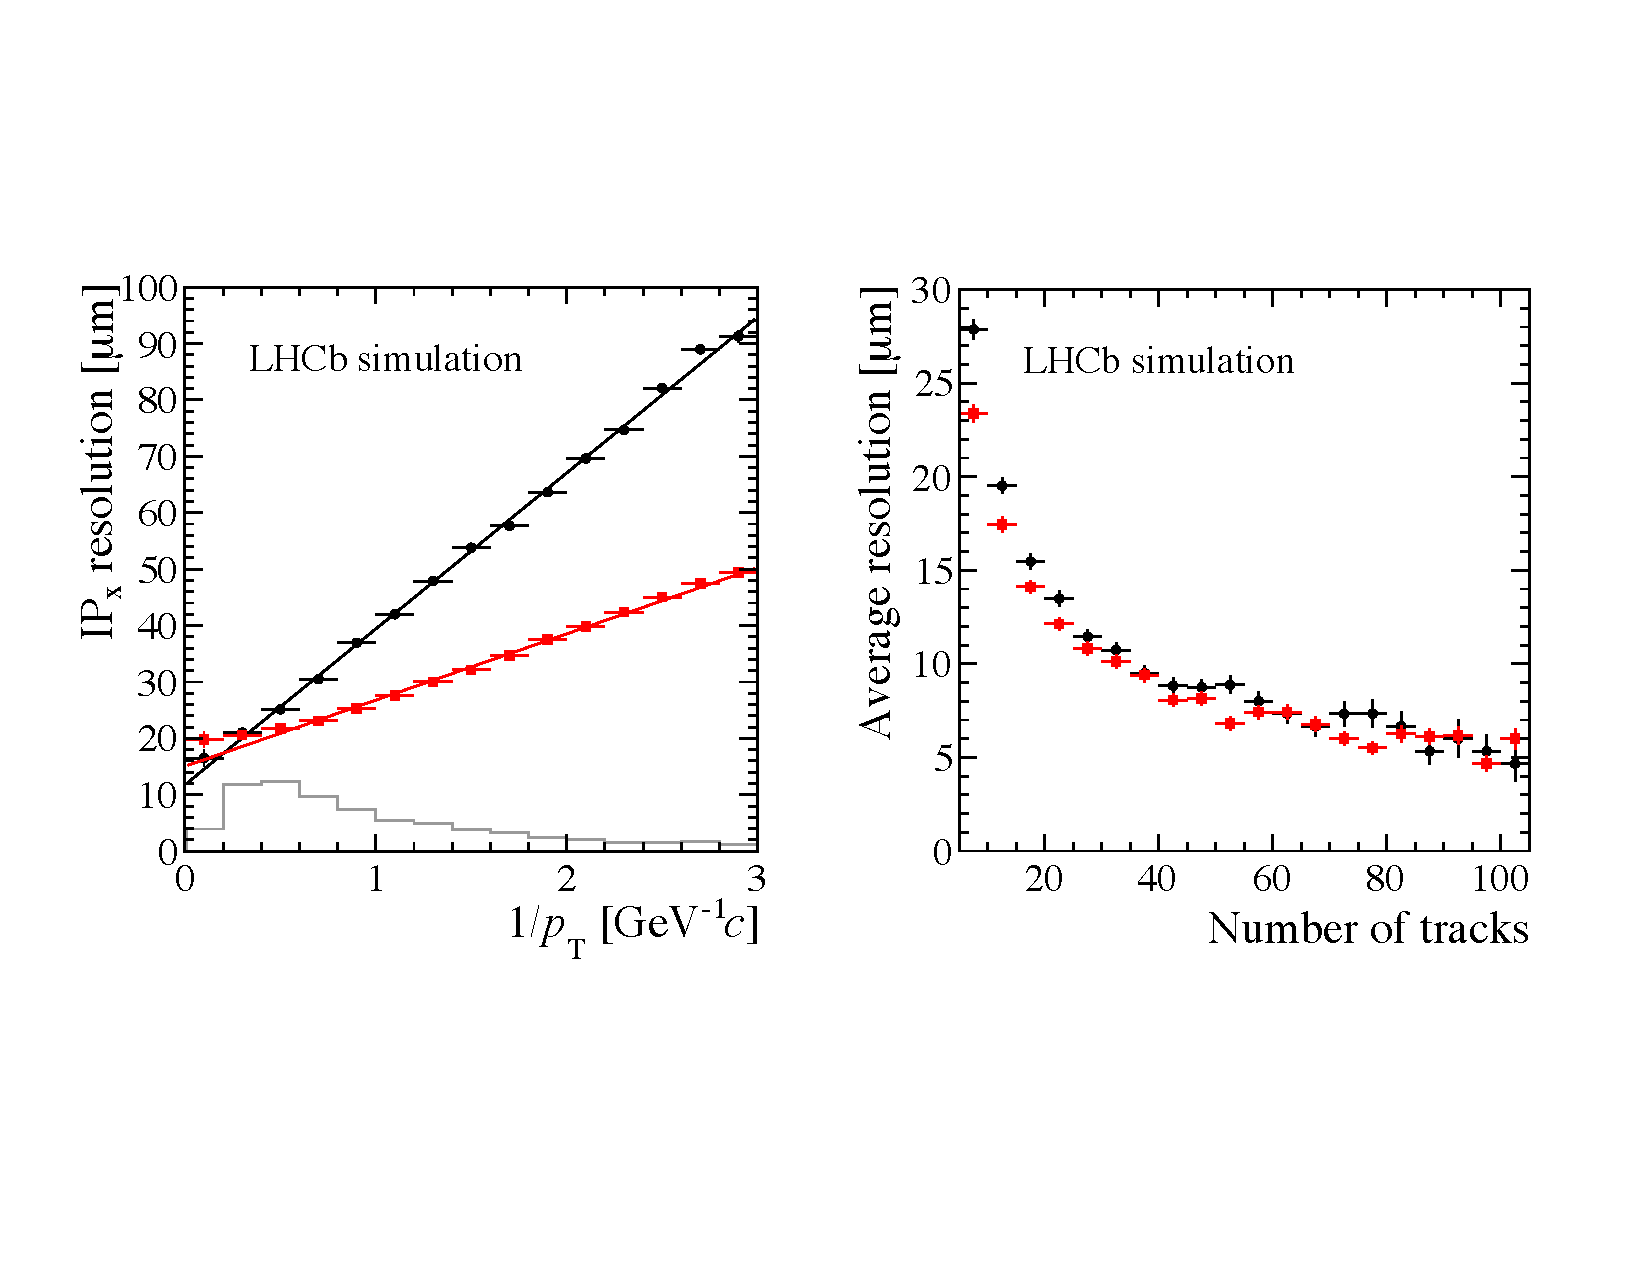
\includegraphics[width=\textwidth]{figures/lhcb_vertexres.pdf}}
  \caption{Resolution of the primary vertex as a function of number of tracks in the $x$ (left) and $z$ (right) direction. The same kind of improvement is also expected for secondary vertices (SV).}
  \label{fig:ulhcb_pvres}
\end{figure}

The pattern recognition efficiency is superior to the one of the current VELO evaluated in upgraded conditions. This can be seen for different observables. Particularly important for LLP searches is the efficiency as a function of the distance from the origin in $z$: for the upgraded VELO, the efficiency approaches $100\%$ and is uniform in a window of 20 cm around the interaction point, thanks to the new configuration of the modules in the $z$ direction and the shorter distance from the beam. After 20 cm in $z$ the VELO acceptance degrades pretty fast, making that the upper limit for LLP decay lengths with vertices reconstructible in the VELO. A display of the upgrade VELO geometry and its acceptance in both forward and backward direction is given in Figure~\ref{fig:ulhcb_veloacc}

Another important figure to evaluate the performance of the detector is the IP resolution, especially in LLP searches where it can be exploited to reduce the background due to fake tracks. With the upgrade the IP resolution significantly significantly improves for low \pt tracks. For example, the IP resolution along $x$ for tracks with \pt of 0.5\gevc is $40\mu{\rm m}$ in the upgrade versus 70 in the current VELO. 
The replacement of strips with pixel sensors also makes the pattern recognition faster for the same multiplicity. This can be used in the trigger to find tracks and identify displaced vertices in the trigger, making it possible to soften or remove inefficient $\pt$ requirements.\\

\begin{figure}[h]
  \centerline{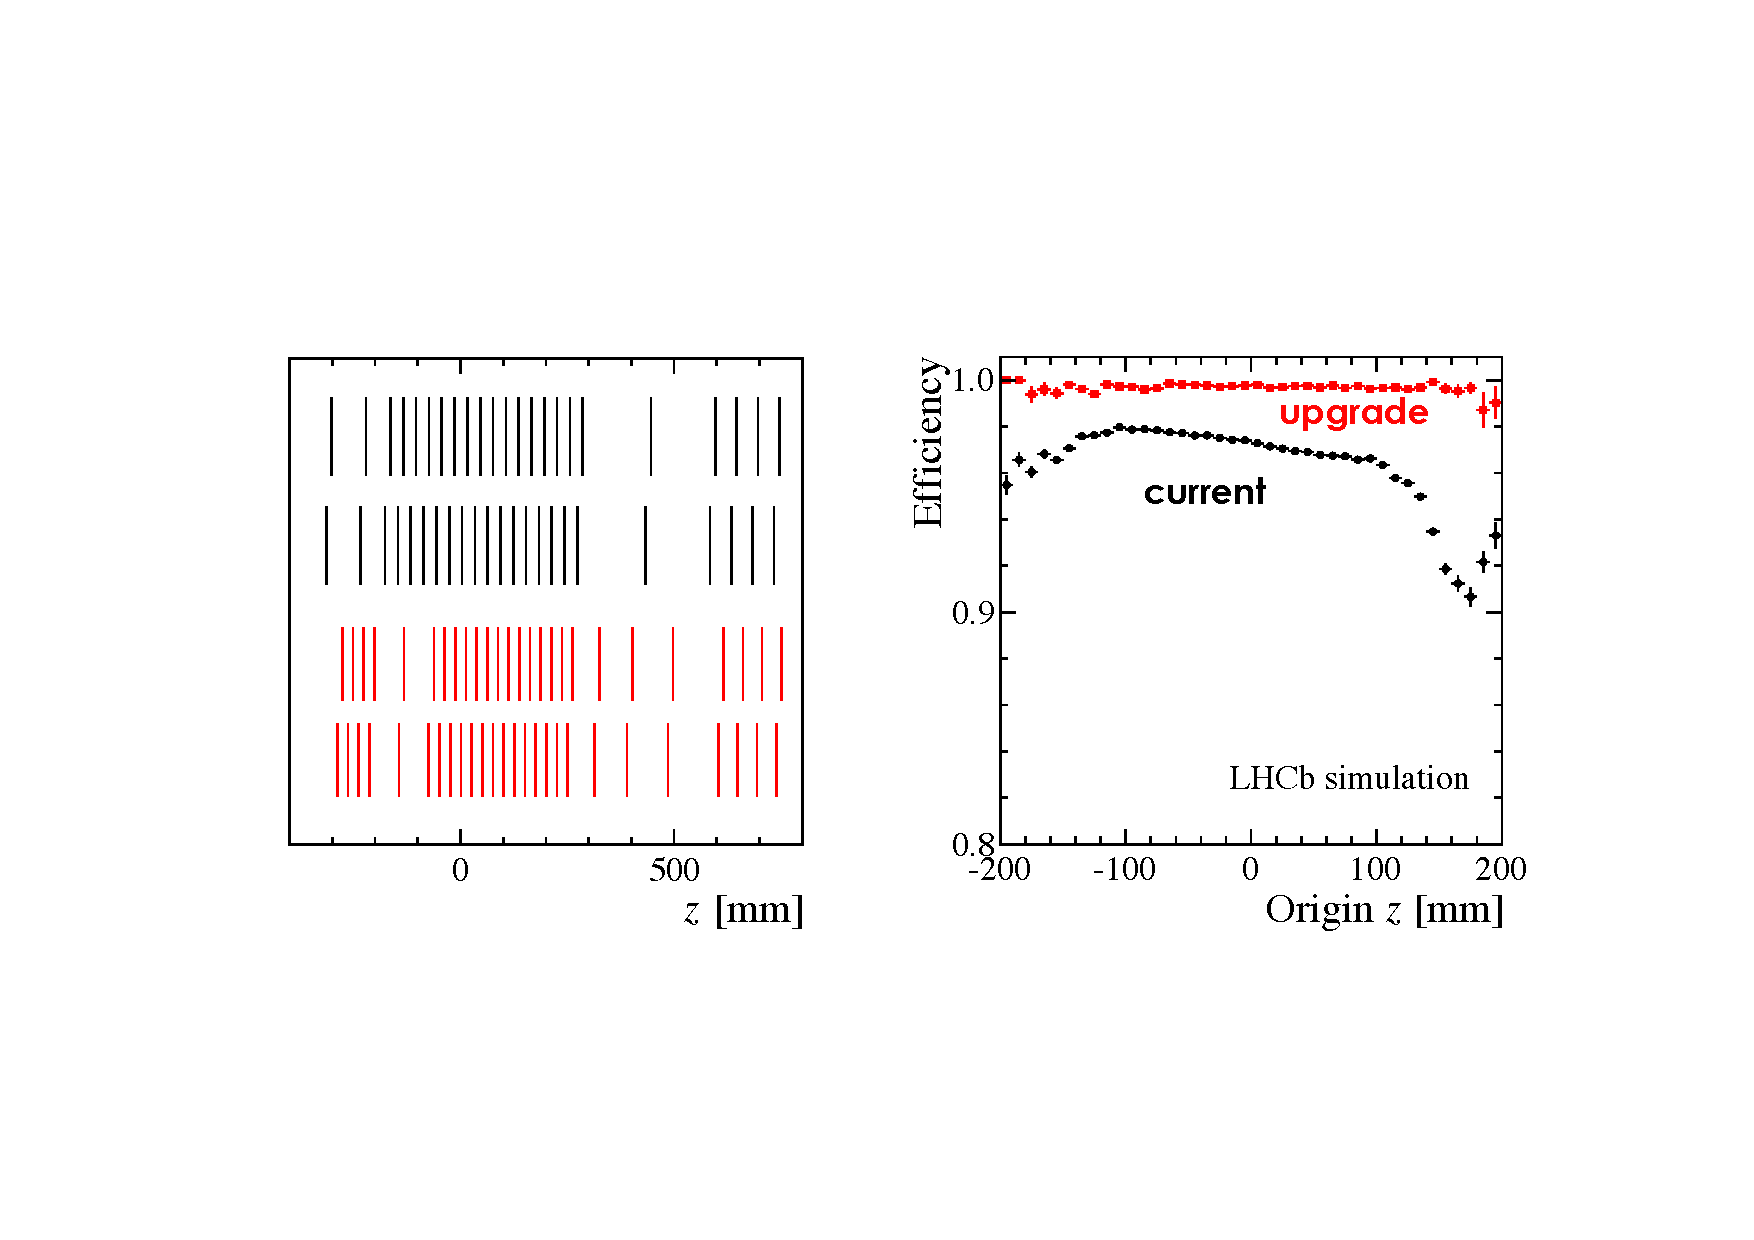
\includegraphics[width=\textwidth]{figures/lhcb_veloperf.pdf}}
  \caption{A comparison of the current and upgrade VELO $z-$layouts is shown on the left. The top layout (black) is the current VELO while the bottom layout (red) is the upgrade VELO. On the right the track reconstruction efficiency is shown as a function of the origin in $z$ for the current (black) and upgrade (black) VELO in upgrade conditions.}
  \label{fig:eff}
\end{figure}

\begin{figure}[h]
\centerline{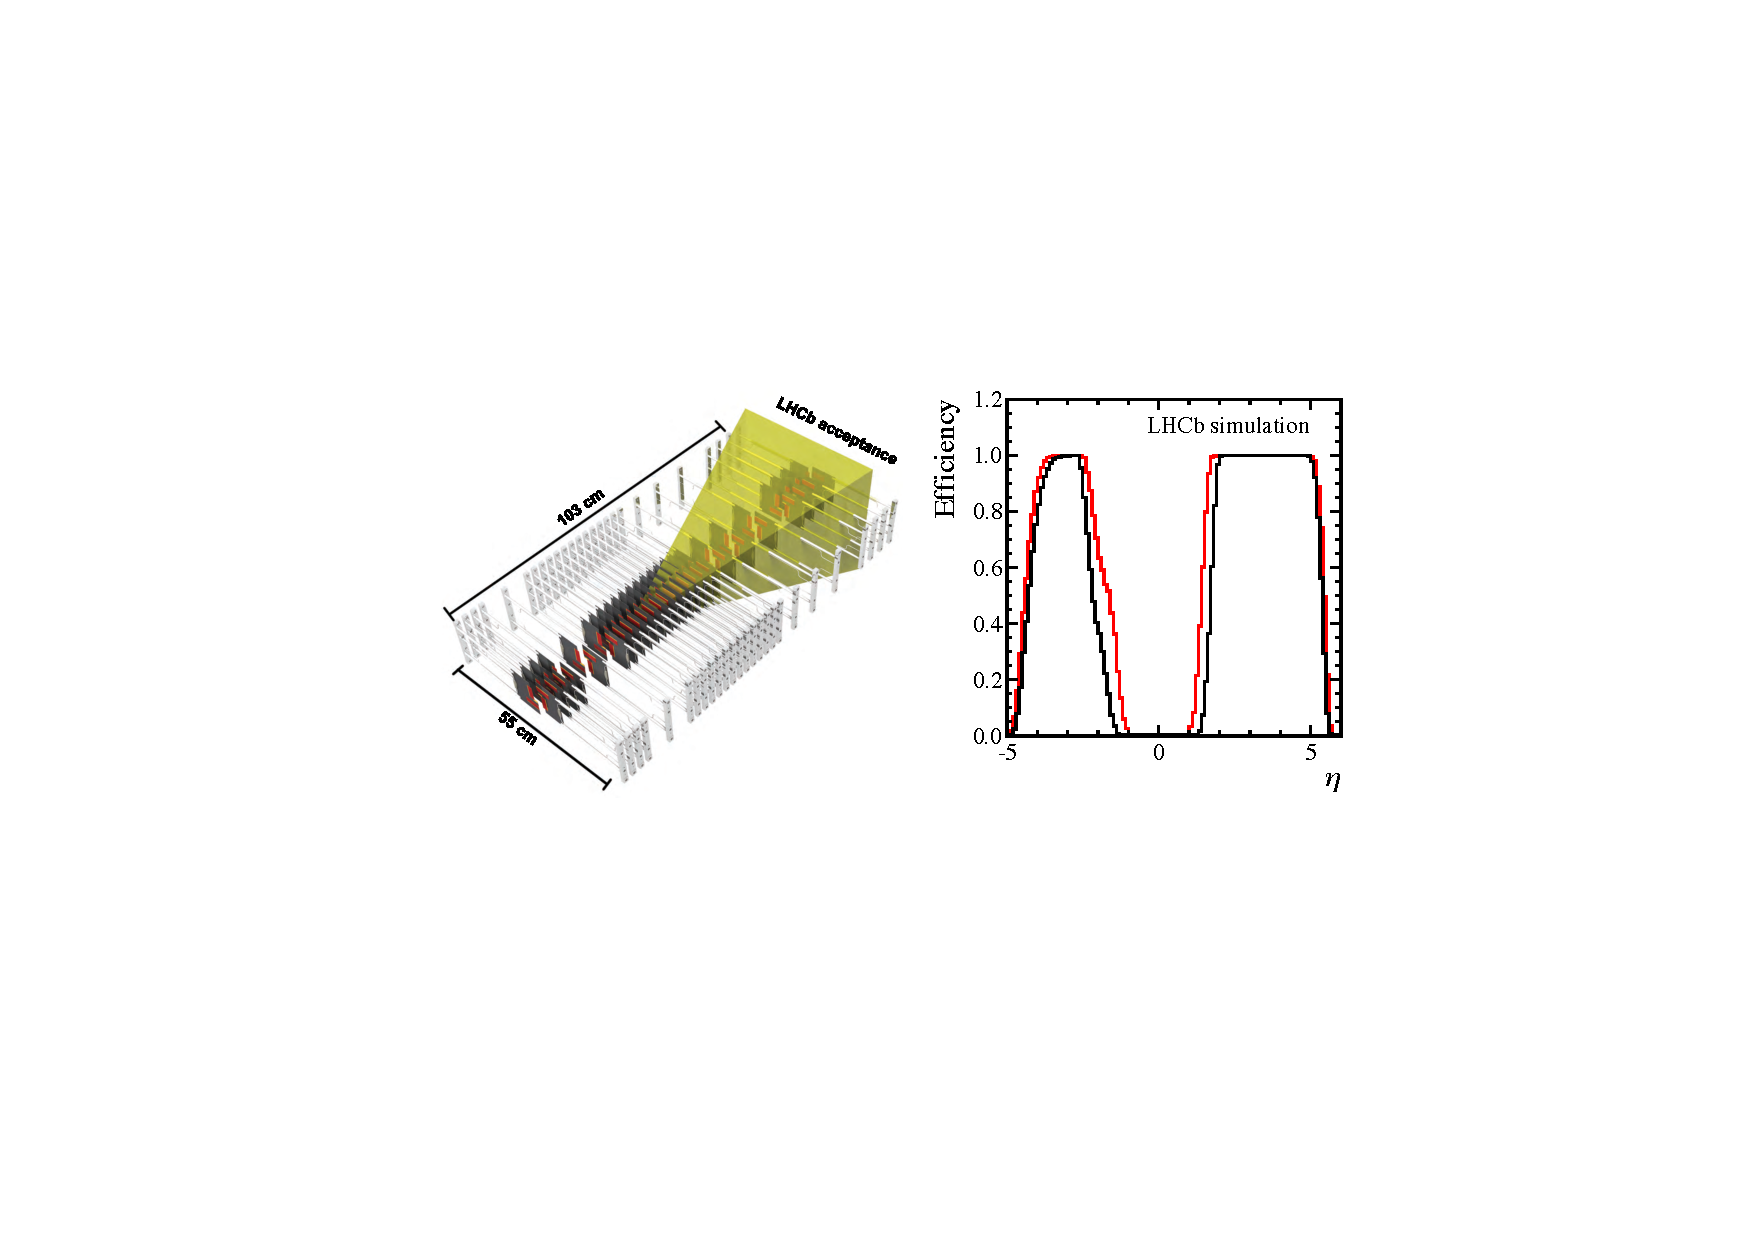
\includegraphics[width=\textwidth]{figures/lhcb_veloacceptance2.pdf}}
  \caption{On the left is a display of the upgrade VELO geometry and a comparison with the LHCb spectrometer acceptance which is shaded in yellow. On the right the $\eta$ acceptance of the upgrade VELO geometry is given both for forward and backward tracks. The fraction of tracks crossing three and four modules is given in red and black, respectively.}
  \label{fig:ulhcb_veloacc}
\end{figure}

Real tracks created in the VELO material can be a significant background to LLP searches (see more details in Appendix~\ref{app:background}. The total material budget of the upgrade VELO is similar to the current one (about $20\%$ radiation lengths) and is dominated by the Radio-Frequency foil separating the beam vacuum from the vacuum of the sensors.
However, the average percentage of radiation length before the first measured point is significantly reduced in the upgrade VELO, passing from $4.6\%X_0$ in the current design to $1.7\%X_0$ in the upgrade VELO.

\subsubsection{Upgraded trigger}

The online event selection in the LHCb experiment during the 2010-2018 running period is performed by a trigger composed of a hardware level (L0), and two software levels, High Level Trigger 1 (HLT1) and the High Level Trigger 2 (HLT2). The L0 reduces the rate from 30 MHz to 1 MHz, using information from the calorimeter and muon systems. Typical thresholds at the L0 are $\pt>1.4\gevc$ for muons and $E>2.5\gev$ for electrons. The software trigger performs a partial event reconstruction at HLT1, reconstructing tracks and primary vertexes for any particle down to $\pt=500\mevc$, followed by complete event reconstruction at HLT2, reducing further the rate to 12.5 kHz (in Run 2).

Given the higher istantenoeus luminosity foreseen after the Phase 1 upgrade, a new trigger system, able to fully exploit the LHC potentiality, has been designed.

The upgraded LHCb trigger consists of two paradigms, a triggerless readout and full software trigger. 
In addition, as already tested in Run 2, a real-time alignment and calibration will allow to achieve offline-quality reconstruction level already in the trigger and a higher signal purity of interesting decay channels. Figure~\ref{fig:ulhcb_trigger} shows the current and the upgrade trigger scheme. 

\paragraph{Triggerless redout and full software trigger}
With the LHCb trigger upgrade the 1 MHz readout limitation will be removed, allowing the full event rate to be processed in software. This will increase the efficiency for several final states which, already in Run 2, cannot benefit from the higher luminosity because of the L0 bottleneck. Figure~\ref{fig:triggervsLumi} shows the saturation for not muonic final state with increasing luminosity.
Moreover, a purely software trigger will not necessitate the tight $\pt$ requirements currently applied at the hardware trigger level. Thanks to this, several physics program involving low-$\pt$ particle, currently prevented because of the low L0 efficiency, will be possible.

\paragraph{Turbo stream}
Starting from Run 2, offline-quality aligment and calibration is applied between the HLT1 and the Hlt2 level. This made possible the design of a new dedicated
trigger output, called Turbo Stream. The event record is written directly from the trigger and processed by the Tesla application~\cite{Aaij:2016rxn}. Its output can be directly used for physics analysis, without the need of offline reconstruction.
Several variation to Turbo have been introduced in the last few years. For the 2015 data taking, the first version of Turbo allowed only the exclusive triggered candidate to be saved, without keeping the rest of the event and discarding all sub-detectors information. 
While the event size was an order of magnitude smaller than for full stream data, any analysis relying on additional infos from the surrounding event could not used Turbo stream data. 
For this reason, in 2016, Turbo++ was implemented, where full event reconstruction was  persisted. Finally, in  2017, a new intermediate solution between Turbo and Turbo++, called Turbo SP (Selective Persistence) was used. With Turbo SP both the trigger candidate and a subset of reconstructed event is saved. This extremely flexible solution allows the analyser to choose which objects to save, minimizing the size of the stored event. A sketch of the evolution of Turbo is showed in Figure~\ref{fig:turbo}.
In view of a full software trigger in the Upgrade, Turbo becomes the only available solution. The reduced event size, would indeed allow to store candidate at high rate, fully exploiting the improvement due to the L0 removal.  


\begin{figure}[h]
\centerline{
 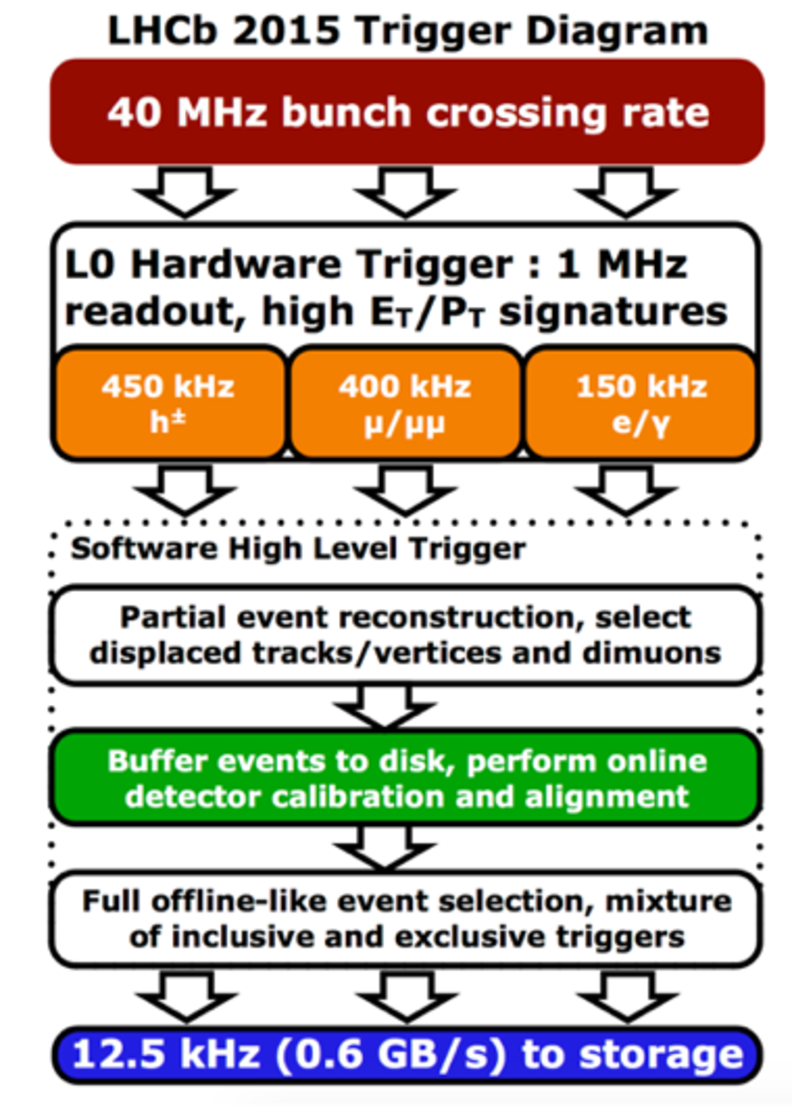
\includegraphics[width=0.5\textwidth]{figures/Trigger2015.pdf}\\
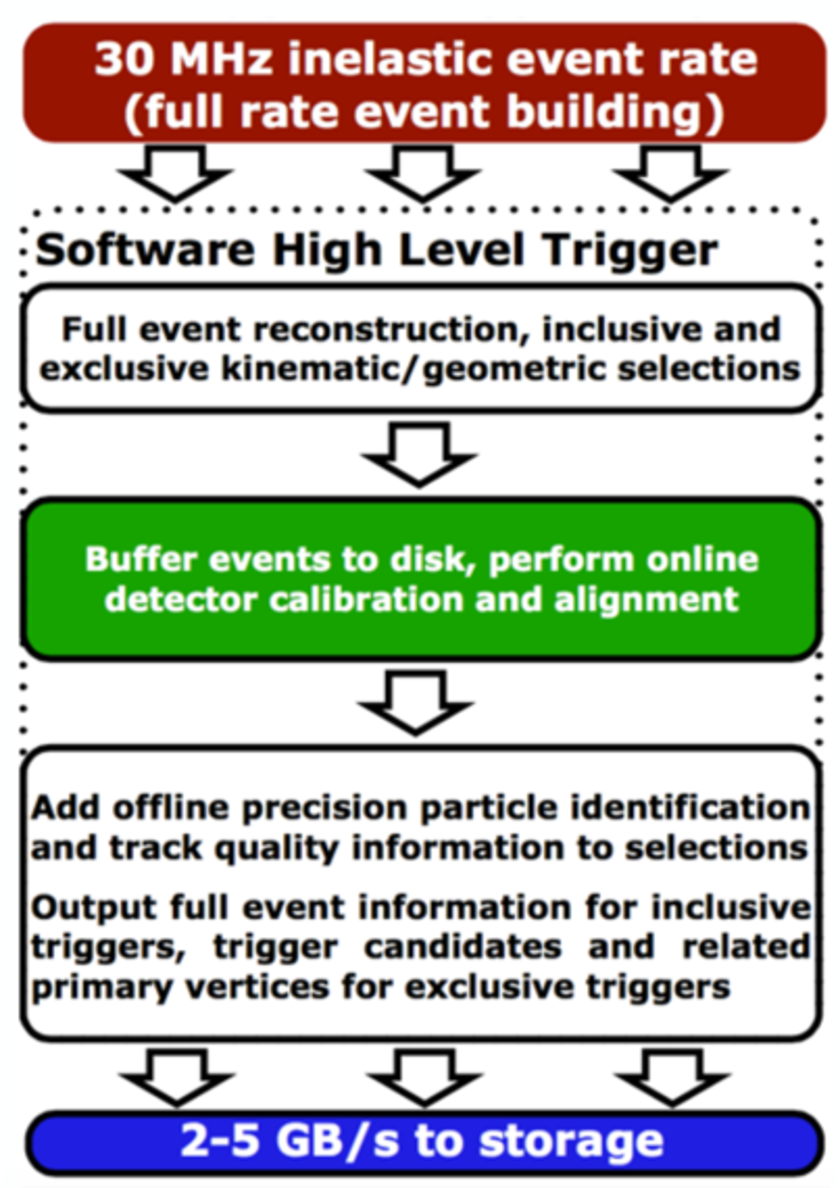
\includegraphics[width=0.5\textwidth]{figures/TriggerUpgrade.pdf}	}
  \caption{Scheme of the current (left) and of the upgraded LHCb trigger scheme (right).}
  \label{fig:ulhcb_trigger}
\end{figure}

\begin{figure}[h]
\centerline{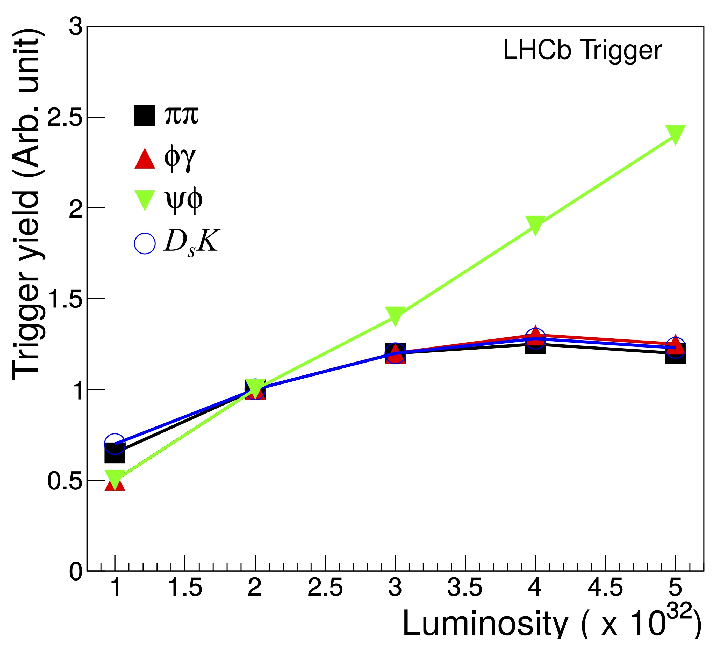
\includegraphics[width=0.6\textwidth]{figures/L0vsLumi.pdf}}
  \caption{Trigger yield as a function of the luminosity. For not muonic channels, the saturation effect due to L0 bottleneck can be observed.}
  \label{fig:triggervsLumi}
\end{figure}

\begin{figure}[h]
\centerline{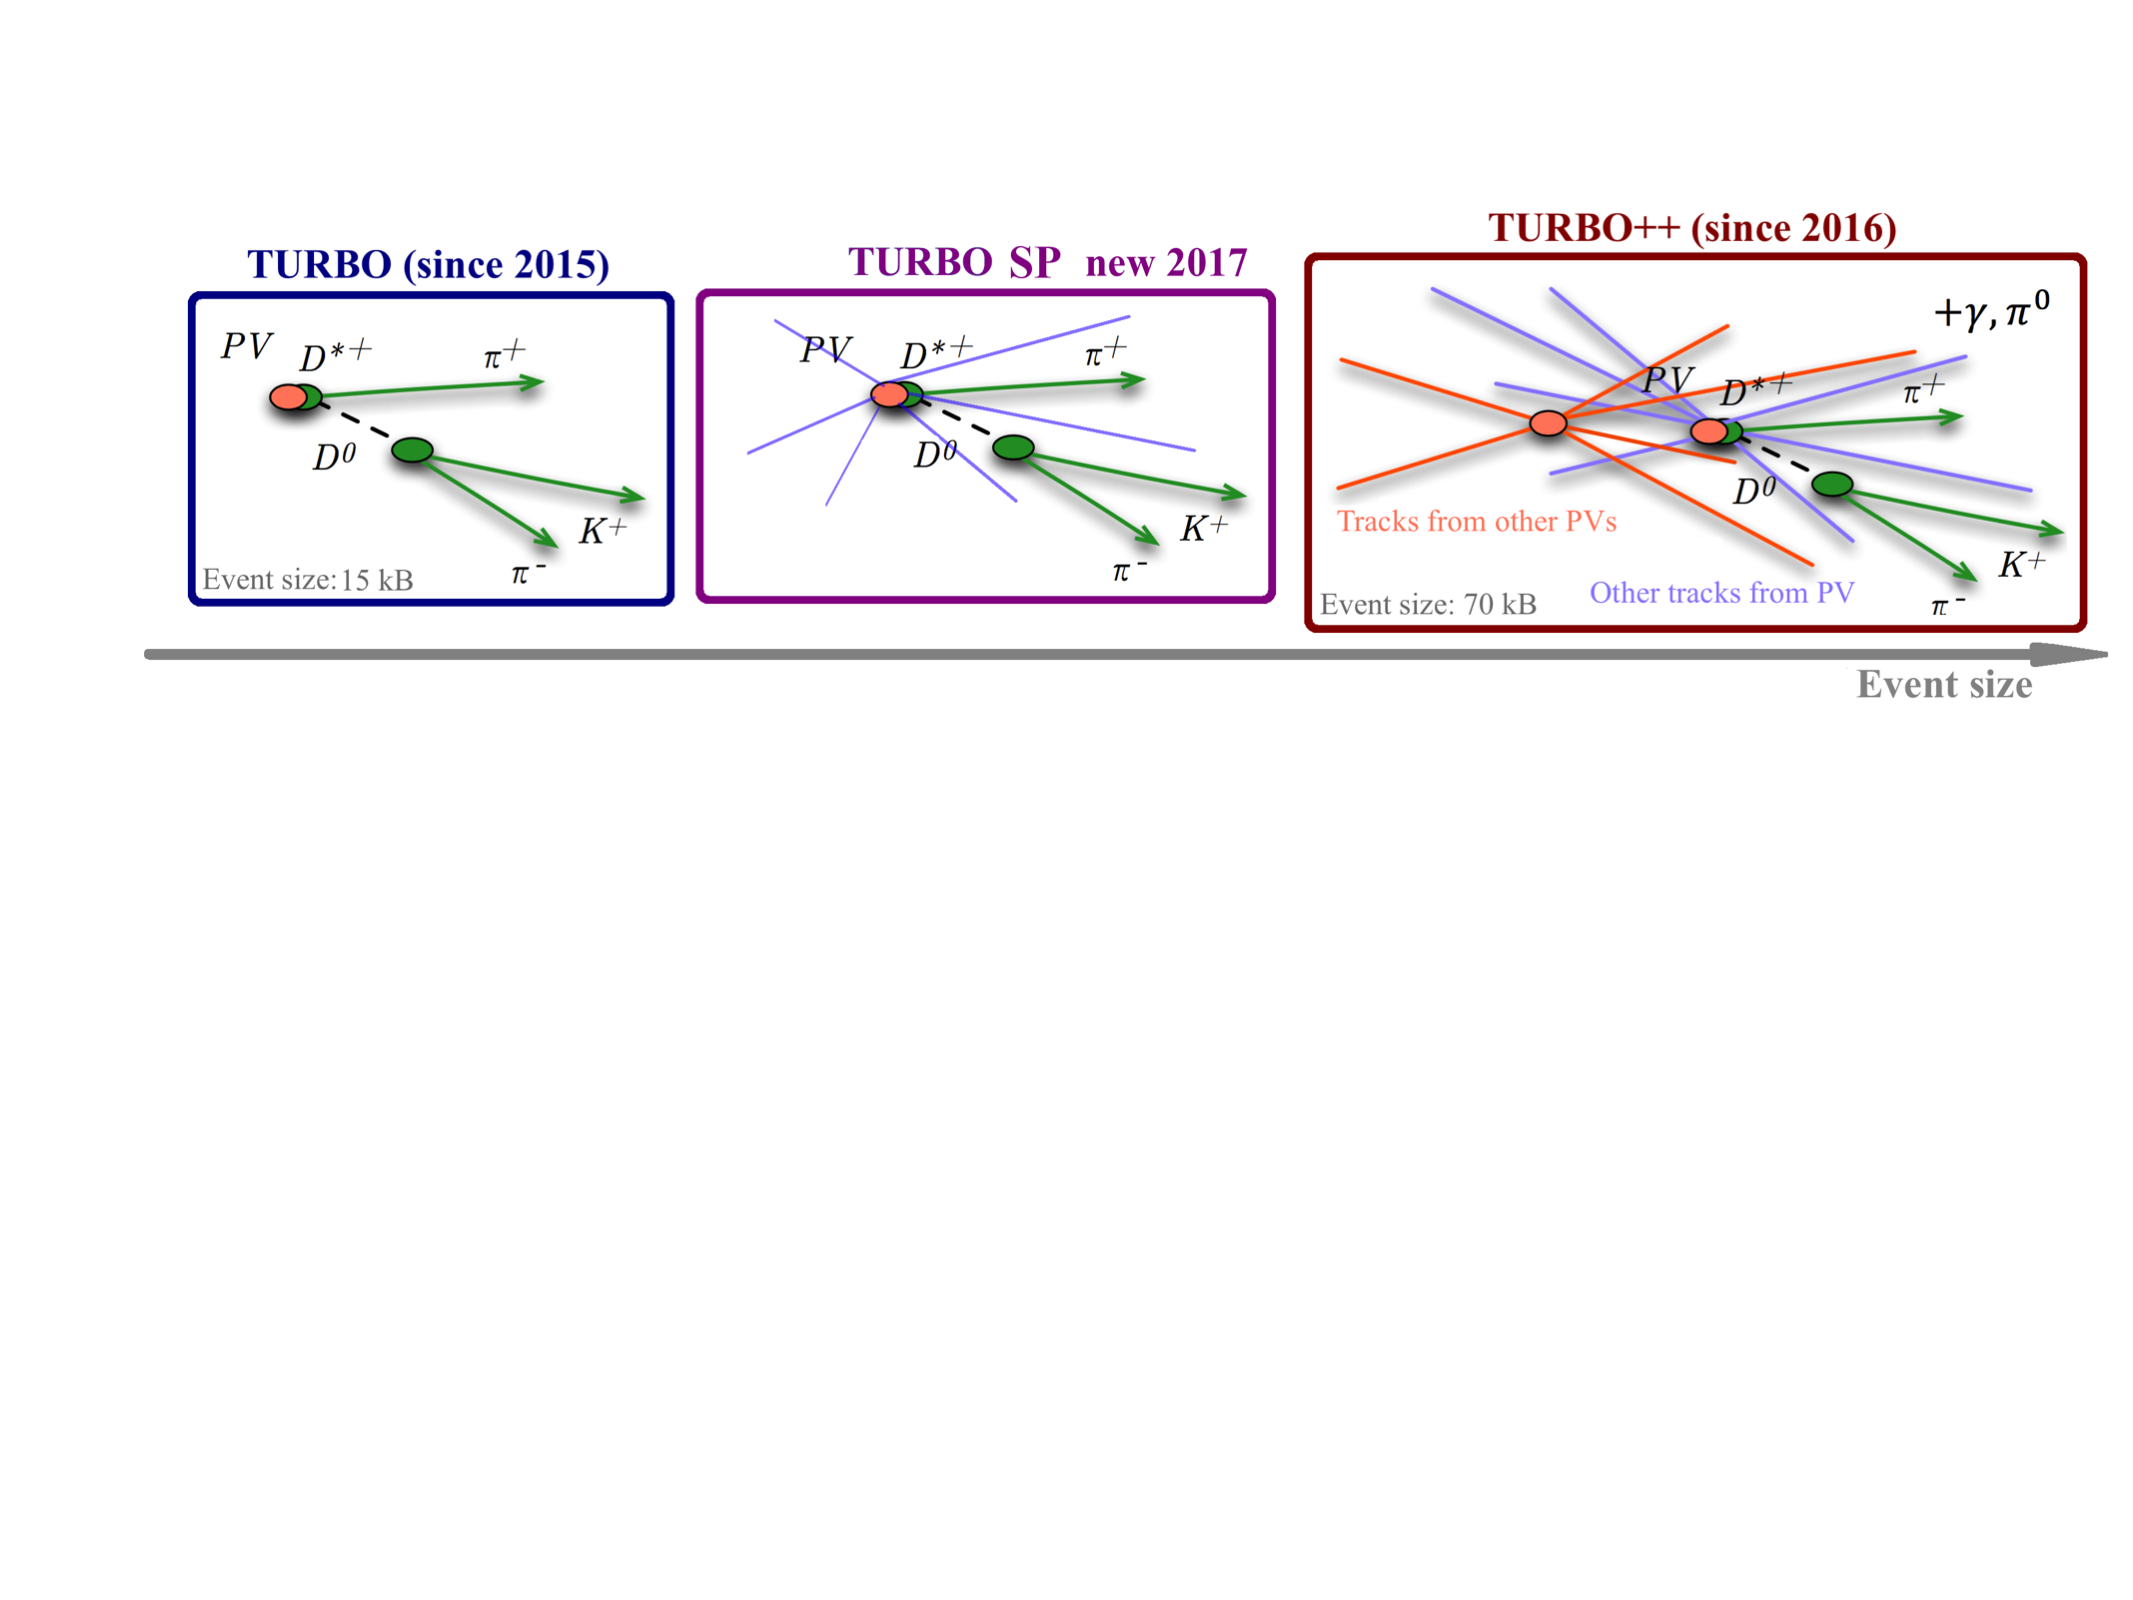
\includegraphics[width=0.95\textwidth]{figures/Turbo.pdf}}
  \caption{Sketch of the evolution of Turbo.}
  \label{fig:turbo}
\end{figure}




\subsection{Upgrade LHCb projections: LLP signatures}
\label{sec:ulhcbphys}

The much higher luminosity and improved capabilities of the upgraded LHCb detector is expected to largely improve the LHCb capabilities in LLP searches in LHC Run 3. In the following, the prospects for a few LLP signatures are given to showcase the upgrade potential. However, the potential of the upgraded trigger-less readout has not been completely explored yet and its great flexibility could be exploited in several ways.

\subsubsection{Displaced di-leptons}
The upgraded LHCb experiment is expected to have exceptional sensitivity to low-mass displaced dilepton signatures thanks to mass resolution, excellent vertexing and the online selection allowed by the trigger-less readout.

The upgrade LHCb sensitivity to dileptons has been explored in the literature in the context of dark photon searches. Two complementary signatures have been considered: an inclusive search for $A'\to \mu\mu$ and a search for using radiative charm decays $D^{*0}\to D^{0}A'(ee)$.
The inclusive search~\cite{Ilten:2016tkc} scans a very large region from the dimuon threshold $2m_{\mu}$ all the way up to the $Z$ pole. The second proposed signature~\cite{Ilten:2015hya} exploits a tag of the radiative decay of the $D^{*0}$ using its reconstructed invariant mass and a dielectron dark photon final state to probe a much lower mass range $[2m_{e}$,142 MeV$]$.
For both signatures, three non-overlapping search regions are defined according to different requirements on the $A'$ flight distance:
\begin{itemize}
\item prompt resonant;
\item displaced upstream of the first VELO module;
\item displaced downstream of the first VELO module.
\end{itemize}
The prompt search is expected to probe mixing parameters $\epsilon^2$ below $10^{-7}$ despite the large irreducible background from Drell-Yan and QCD.
Since the search for displaced dark photons is not expected to exclude a physical parameter above the $\eta$ mass, no attempt is made to probe that region.

An inclusive search has already been performed with Run 2 data~\cite{Aaij:2017rft}. This has been possible thanks to the high reconstruction and identification efficiency of soft di-muons at LHCb. These results demonstrated the unique sensitivity that can be reached at LHCb. The planned increase in luminosity and removal of the hardware- trigger stage in Run 3 should increase the number of expected $A'\to \mu\mu$ decays in the low-mass region by a factor of ${\cal O}(100-1000)$ compared to the 2016 data sample. The limits placed by the current data and the sensitivity expected with future LHC runs is shown in Figure~\ref{fig:lhcb_darkph}.

On the other side, the exclusive search is much more challenging and not feasible prior to the upgrade, since the hardware trigger and the thicker RF foil degrade the sensitivity. This search highly relies on the online identification of $e^{-}e^{+}$ pairs, since over 5 trillions decays are expected in Run 3. The expected sensitivity probes unexplored regions of phase space at very low $A'$ mass and mixing $\epsilon^2$ which is usually the realm of beam-dump experiments.
\begin{figure}[h]
  \centerline{\includegraphics[width=\textwidth]{figures/lhcb_darkphoton_projections.pdf}}
  \caption{Current and expected limits in the dark photon parameter space mixing $\epsilon^2$ versus $A'$ mass. Blue-shaded limits are the current LHCb limits from~\cite{Aaij:2017rft} while grey-shaded ones are existing limits from other experiments. The dashed azure line represents the naive expected limit for the search that was performed with 13 TeV collisions~\cite{Aaij:2017rft}: it agrees fairly well with the observed limits. Limits from the proposed inclusive search with 15, 50 and 500 \invfb are shown in progressively darker red. The expected sensitivity of $D^{*0}\to D^{0}A'(ee)$ at low mass are shown in progressively darker green for 15, 50 and 300 \invfb.}
  \label{fig:lhcb_darkph}
\end{figure}

A displaced dimuon signature also appears in some hidden-valley scenarios where dark mesons have a large enough decay rate to leptons. The upgrade LHCb prospects for this kind of signature have been explored in~\cite{Pierce:2017taw} and are extremely promising.
In the scenario explored in~\cite{Pierce:2017taw} dark mesons are produced with large multiplicities between 10 and 30 and selection criteria borrowed from the proposed dark photon search~\cite{Ilten:2016tkc} in the region after the first VELO module.
The expected reach for the proposed searches using Run 3 data from LHCb (15\invfb) and from ATLAS/CMS (300\invfb) are shown in Figure~\ref{fig:ulhcb_hv_dimuons}. The model studied involves a 200\gevcc $U(1)'$ gauge boson $Z_p$ decaying to a hidden-valley quark pair; showering and hadronization in the dark sector leads to a large multiplicity of hidden hadrons $\omega_V$ (with $m_{\omega_V} =0.3\gevcc$) that can decay to dimuons. In this context the upgrade LHCb could have better sensitivity than other proposed searches at ATLAS and CMS. 

\begin{figure}[h]
  \centering
  {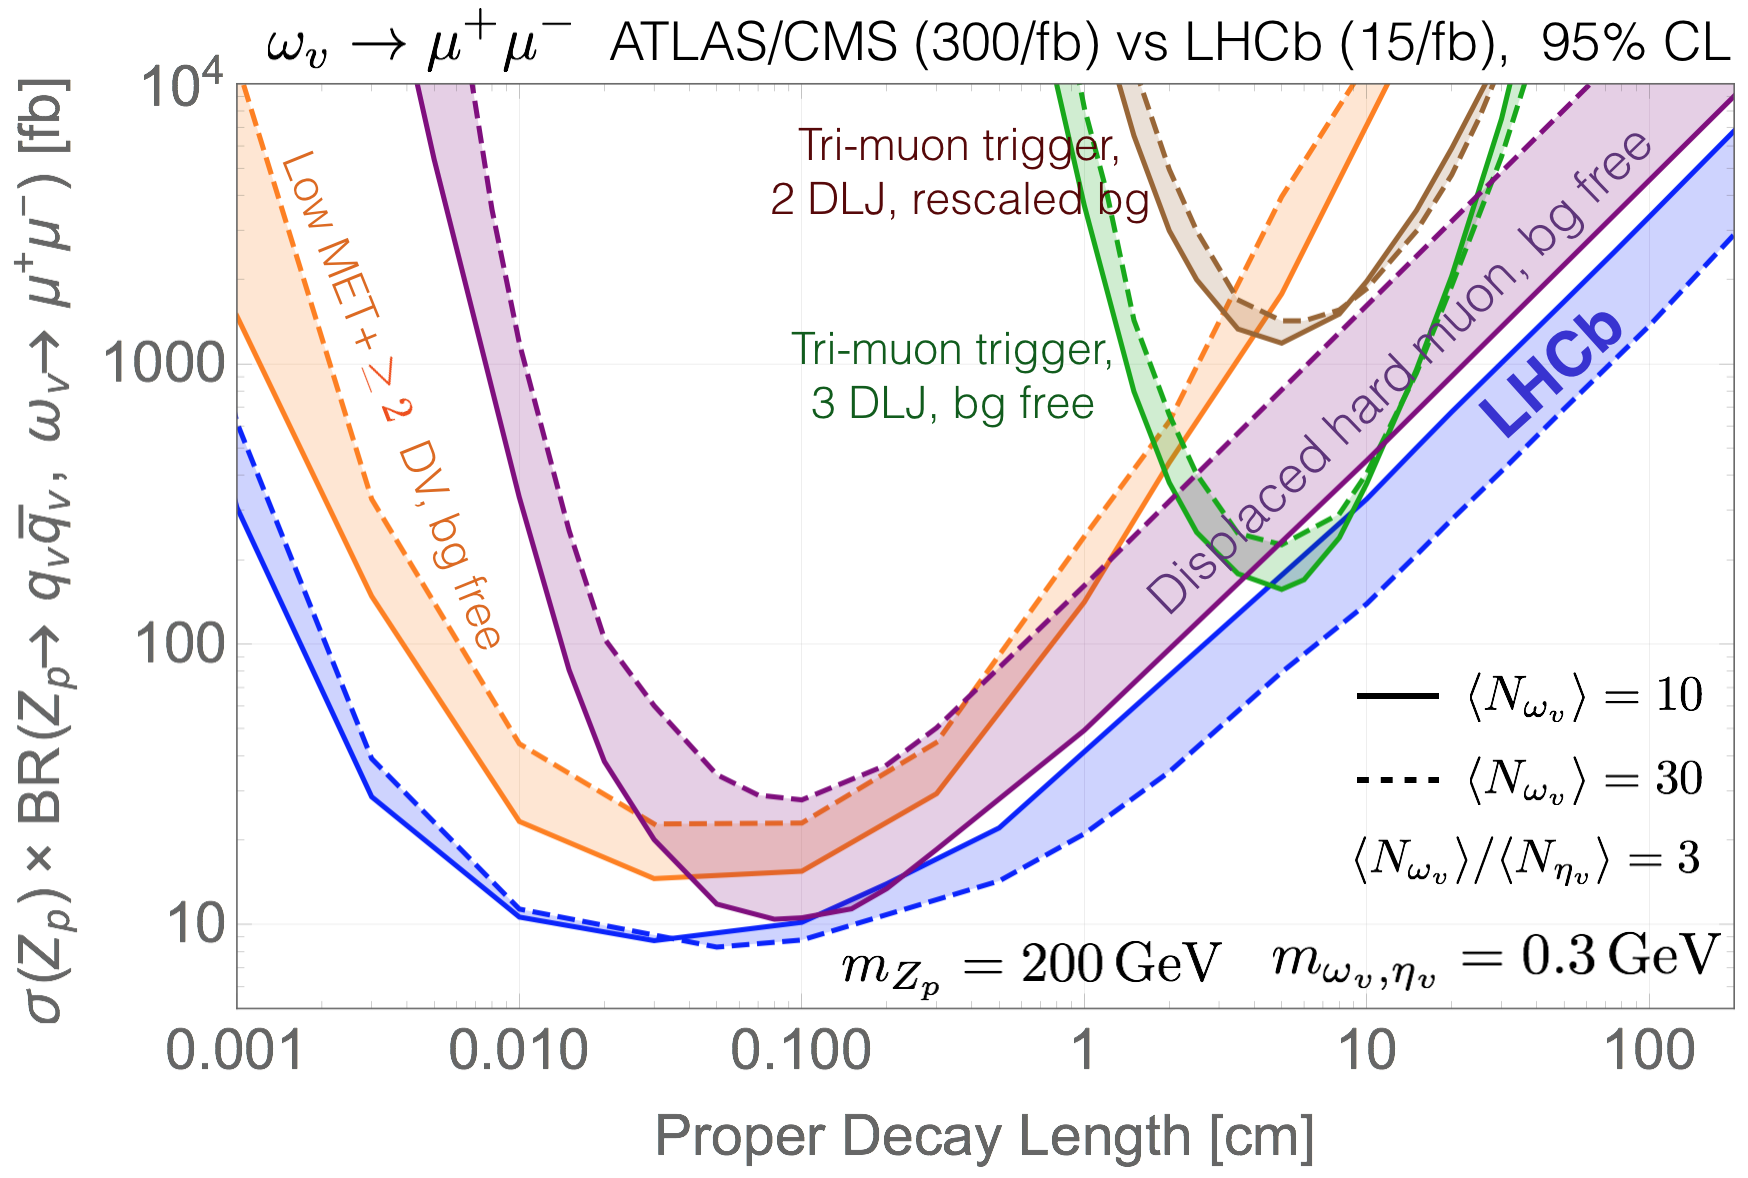
\includegraphics[width=0.8\textwidth]{figures/ulhcb_darkmesons_dileptons.png}}
  \caption{Projected bounds from various ATLAS/CMS searches and the LHCb search for the di-muon~\cite{Pierce:2017taw}.}
  \label{fig:ulhcb_hv_dimuons}
\end{figure}


\subsubsection{Displaced jets}
Signatures with displaced jets are very common in the context of long-lived particle searches. LHCb has already started to explore its potential by using the data collected during Run 1 to search for the following signatures: a single~\cite{Aaij:2017mic} and a double~\cite{Aaij:2016isa} displaced di-jet and a single displaced high-multiplicity vertex including a high$-\pt$ muon~\cite{Aaij:2016xmb}. 
Starting with the former signature, already in Run 1 limits have been set on dark sector V-pions from Higgs decaying to quark-antiquark pairs. 

In the upgrade LHCb, the background rejection for displaced jet searches is expected to improve thanks to the improved VELO resolution and the selection efficiency should be significantly higher thanks to the online displaced vertex identification. 
The main focus of LHCb will be to probe the region at very low lifetime where it has already probed to be most competitive (see discussion in EXPERIMENTAL COVERAGE CHAPTER). There, the background from QCD and material interactions is the main limiting factor and the improved vertex resolution of the upgrade VELO together with the lower material budget and the use of a detailed material map are expected to bring large improvements.

In some dark sector models the number of displaced vertices can be very large, even in the limited LHCb acceptance~\cite{Schwaller:2015gea}. Typical displaced vertex searches would probably discard these events due to requirements on vertex isolation that are used to remove fake signatures, so a dedicated search strategy is needed. Furthermore, a dedicated software trigger looking for a large number of displaced vertices in the VELO and very soft $\pt$ requirements could in principle be very sensitive to this kind of models, but studies are needed to fully understand its potential and compare it to other experiments.

\subsubsection{Displaced mesons}
SM quark-antiquark pairs from the decay of a low mass particle can often hadronize in SM mesons that subsequently decay with known branching ratios. For example a dark-sector meson with a displaced decay to $c\bar{c}$ often produces two $D$ mesons which in turn have a non-negligible lifetime. In this scenario, the authors of ~\cite{Pierce:2017taw} have investigated the prospects of using more or less inclusive reconstruction of the two $D$ mesons decays at the upgraded LHCb. A very similar approach could be used to target decays to $b\bar{b}$ that hadronize to $B$ mesons since the latter is very likely to produce $D$ mesons in its decay. Since LHCb is designed to reconstruct heavy flavour decays, it can be very competitive in this kind of searches as it was shown in~\cite{Pierce:2017taw}. Furthermore, this kind of search will greatly profit from the software trigger which is mainly designed to improve the efficiency of this kind of hadronic decays of heavy flavour mesons.

\begin{figure}[h]
  \centering
  {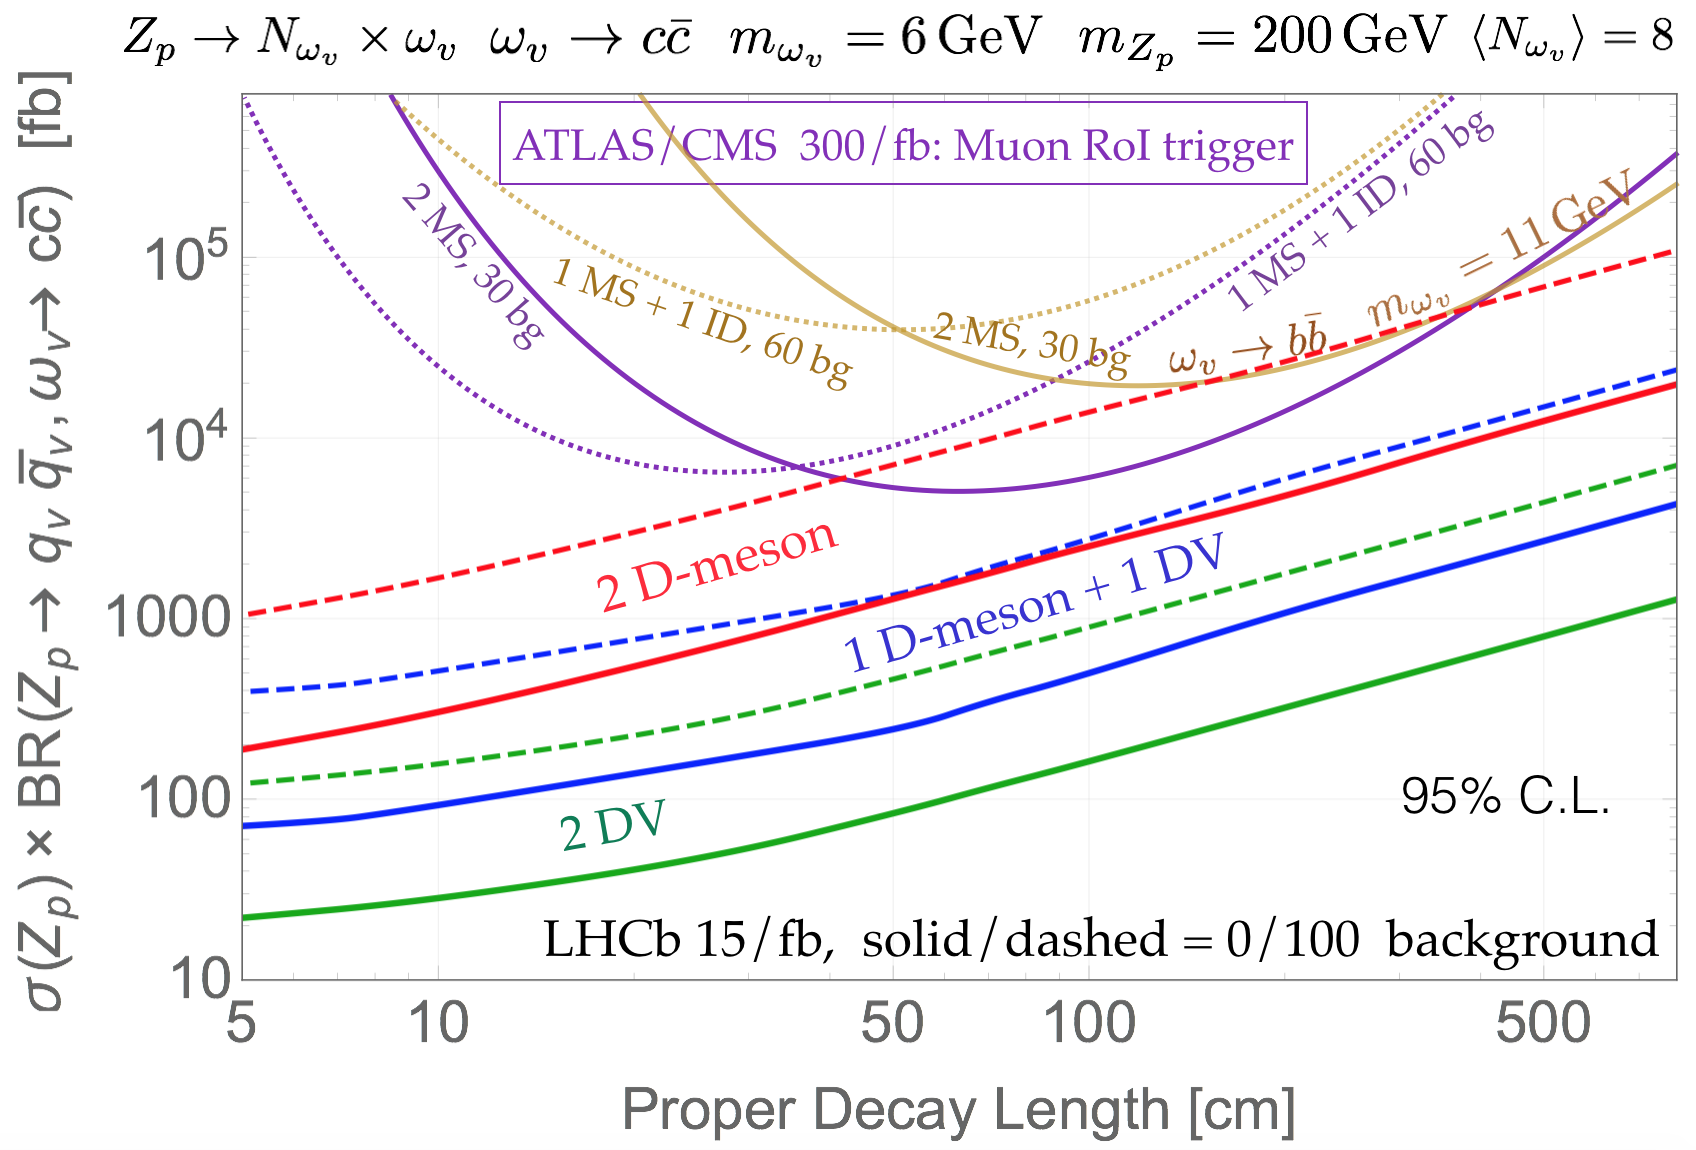
\includegraphics[width=0.8\textwidth]{figures/lhcb_hvlimits2.png}}
  \caption{Projected bounds from various proposed searches for confining hidden valley models exploiting $c\bar{c}$ decays of hidden valley mesons $\omega_v$ taken from~\cite{Pierce:2017taw}. The sensitivities with various signatures at LHCb are shown: two displaced vertices (green), one reconstructed $D$ meson and one DV (blue) and two reconstructed $D$ mesons (red). Searches for this same partiular model at ATLAS/CMS are shown not to be competitive (more details can be found in ~\cite{Pierce:2017taw}).}
  \label{fig:HVlim}
\end{figure}

\subsection{After Phase-I upgrade: Phase-II and more}
TO BE FILLED WITH SOME PROSPECTS AND NEW IDEAS
\label{sec:ulhcbphaseii}
\begin{itemize}
\item downstream triggers for displacements larger than 20 cm
\item removal of RF foil to reduce VELO material interaction background
\item dedicated ASICs for downstream tracking embedded in DAQ
\item Tracking chambers inside the magnet for low momentum particles (useful for soft pion from ``disappearing'' chargino track?)
\end{itemize}

\begin{figure}[h]
\centerline{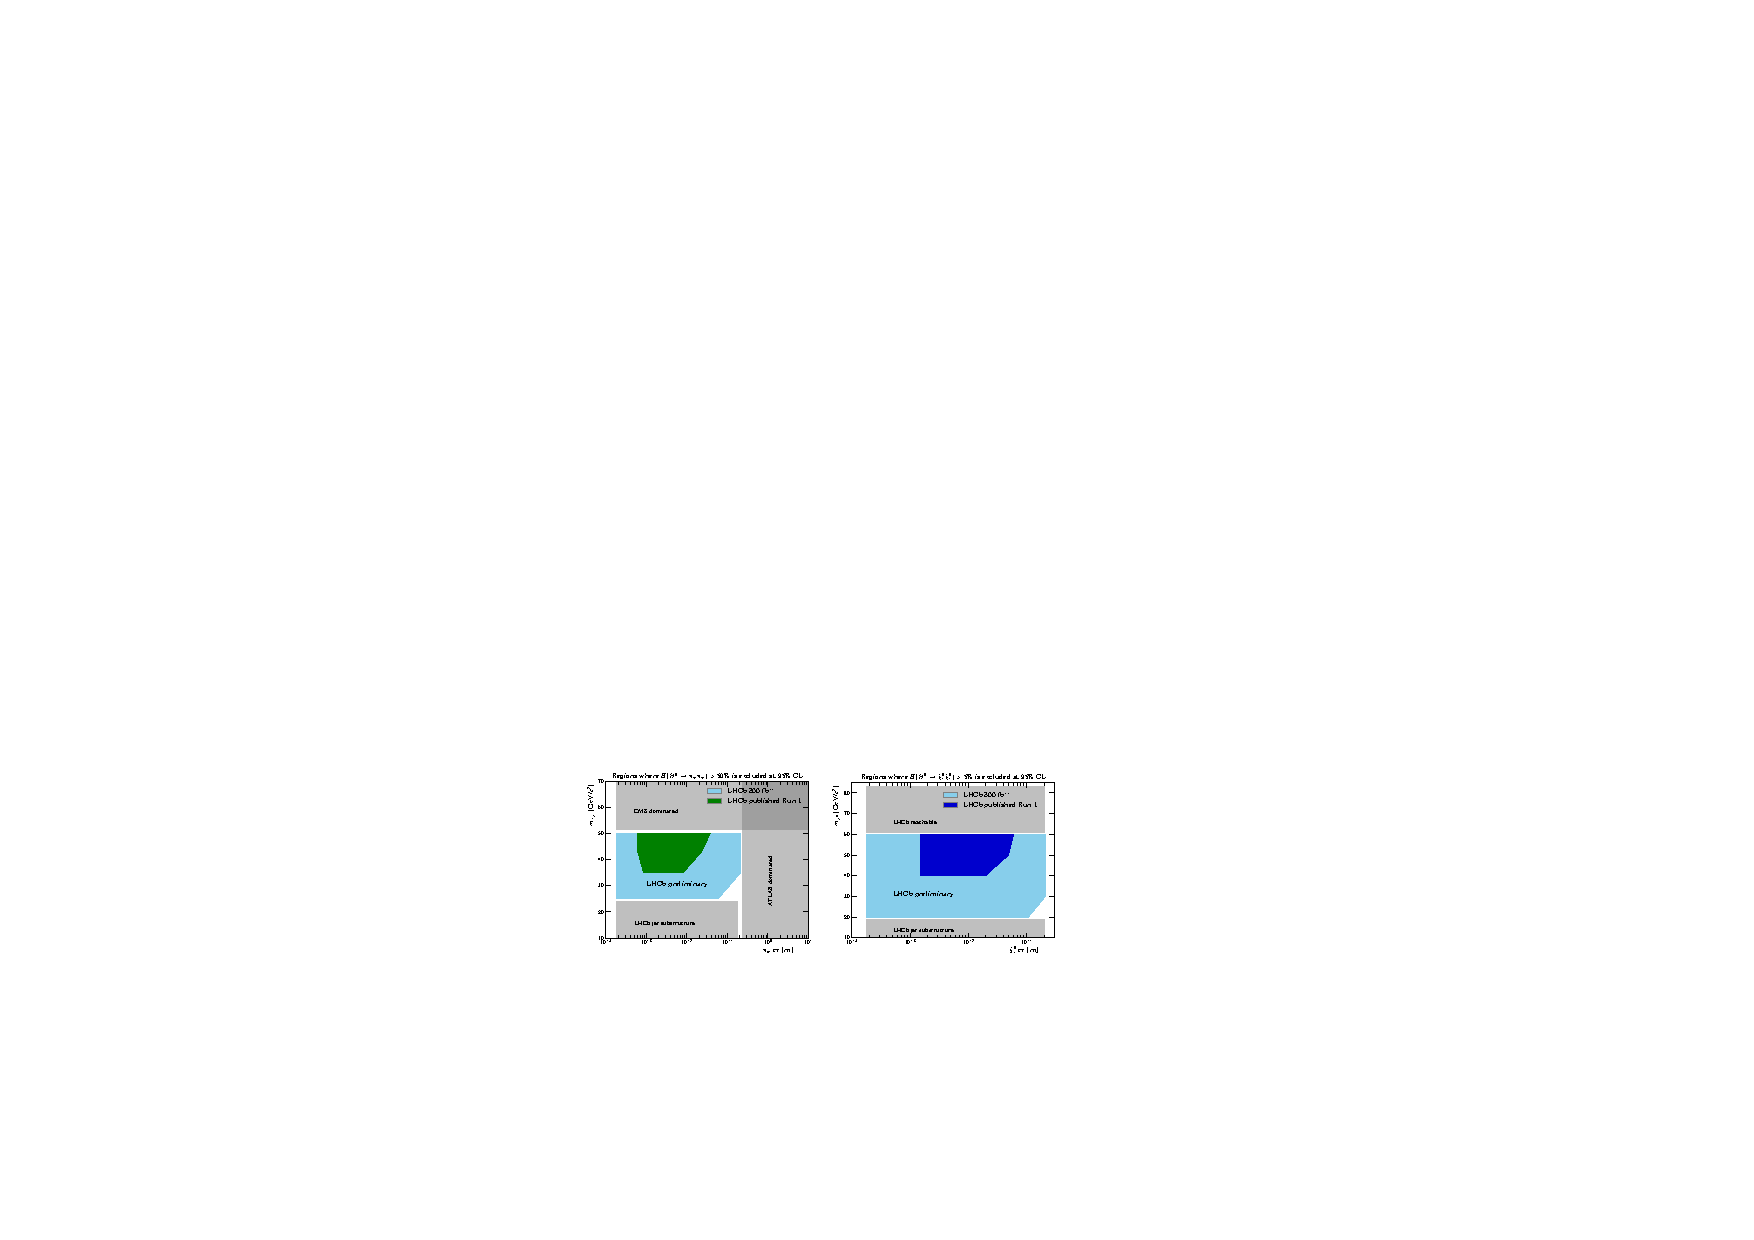
\includegraphics[width=0.95\textwidth]{figures/p2lhcb_dvsearches.pdf}}
  \caption{Naive projections of Run 1 results from searches of displaced jets at LHCb to the expected luminosity to be collected with the Phase-II upgraded detector. On the left is the projection of the search for a single displaced dijet~\cite{Aaij:2017mic} while on the right is the one for a single displaced vertex with a high$-\pt$ muon~\cite{Aaij:2016xmb}.}
  \label{fig:ulhcb_trigger}
\end{figure}

